\documentclass[../Book.tex]{subfiles}
\usepackage{subfiles}

\begin{document}
\chapter{Tabla Hash}
En el capítulo anterior, hemos examinado varias técnicas de búsqueda. Considere un problema de buscar un valor en una matriz. Si la matriz no se ordena, no tenemos otra opción, sino que busque en cada elemento uno por uno, por lo que la complejidad de la hora de búsqueda será O (N). Si la matriz está ordenada, podemos buscar el valor que estamos buscando en O(logn) Tiempo logarítmico usando la búsqueda binaria.	
\\
¿Qué sucede si tenemos una función que puede decirnos la ubicación / índice del valor que estamos buscando en la matriz?
Podemos ingresar directamente a esa ubicación y decir si nuestro objeto que estamos buscando está presente o no en solo O (1) tiempo constante. Dicha función se llama una función de hash.
\\
En la vida real, cuando se entrega una carta a un cartero, el al  observar la dirección en la carta sabe con precisión a que casa necesita ir. El no tendra que tocar de puerta en puerta para saber de quien es.
\begin{figure}[htb]
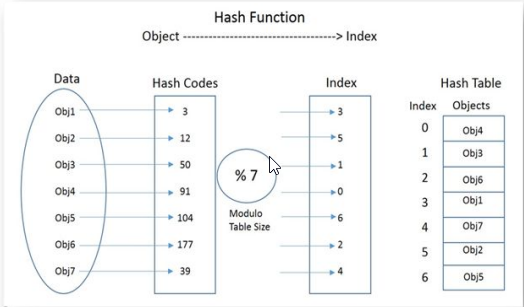
\includegraphics{Tabla Hash Ejemplo}	
\caption{\label{fig:TablaHashEjemplo} Es una ejemplo de la tabla hash.}
\end{figure}
El processo de almacenamiento de objetos usando una función hash es el siguiente:
\begin{enumerate}
\item Crea un arreglo de tamaño M para almacenar los objetos, este arreglo sera llamado Tabla Hash.
\item Encuentra un código hash de un objecto pasando este a traves de la función hash.
\item Toma el modulo del codigo hash por el tamaño de la tabla hash para obtener el indice de la tabla donde los objetos serán almacenados.
\item Finalmente almacena esos objetos en el indice designado.  
\end{enumerate}

El proceso de busqueda de objetos en la tabla hash usando una función hash es el siguiente:

\begin{enumerate}
\item Encuentra un codigo hash del objecto que se esta buscando pasando como argumento a la función hash.
\item Toma el modilo de el código hash por el tamaño de la tabla hash para obtener el indice de la tabla donde se almacenaron los objetos.
\item  Finalmente,  recupera el objeto del índice designado
\end{enumerate}
\subsection{Tabla Hash}
Una tabla hash es una estructura de datos, cual contiene claves de mapa a valores. Cada posición de la tabla hash es llamada espacio(slot). La tabla has usa una función hash para calcular un indice de un arreglo de espacios. Usaremos la tabla hash cuando el numero de claves almacenadas sea mas pequeño que el numero de posibles claves.

\subsubsection{Tabla hash con typo de dato abstracto}
Un tipo de dato abstracto de la tabla hash contiene las siguientes funciones.
\begin{enumerate}
\item Insert(x) añade el objeto al conjunto de datos.
\item Delete(x), elimina el objeto x de el conjunto de datos.
\item Buscar(x), busca el objeto x en el conjunto de datos.
\end{enumerate}
\subsubsection{Función Hash}
Una función hash es una función, el cual genera unindice en una tabla para dar un objeto.

Una función Hash ideal debe generar un unico indice para cualquier objeto, suele llamarse función hash perfecta.
\textbf{Programa Hash Function Simple}
Hay muchas funciones hash, pero esta es lo minimo que debería hacer. Varias generaciones lógicas de hash serán añadidas a esta función para generar mejores hash.
\subsection{Propiedades de una buena función Hash}
\subsection{Factor de Carga}


\end{document}